


\section{Experiments}

In order to evaluate the effects of different components in SOVI and compare it with state-of-the-art approaches, we conduct series of comparative test and ablation study on two datasets, YouTubeVOS \cite{xu2018Youtube} and DAVIS \cite{davis_2017}.
%We test on two datasets, YouTubeVOS \cite{xu2018youtube} and DAVIS \cite{davis_2017}, to compare the proposed STSENet with state-of-the-art methods. %Several ablation studies are conducted to prove the effectiveness of spatial details and temporal information in video inpainting.
%\subsection{Experimental Settings}

\noindent\textbf{Dataset.} 
YouTubeVOS and DAVIS are widely used for evaluating video inpainting results in recent studies.
YouTubeVOS consists of 4,453 video clips that contains more than 70 categories of common objects. 
The videos are split into three parts, 3,471 for training, 474 for validating, and 508 for testing.
% 
DAVIS dataset contains 90 video sequences that are annotated with foreground object masks and 60 unlabeled videos for training. 


\dlt{
is for video object segmentation containing 150 video clips, among which 60 randomly sampled clips are for testing of object removal. And the rest part is used for training.
The videos are complex with occlusions, fast motion, and various objects. }

\noindent \textbf{Mask Setting.} Considering different real-world applications, we test four kinds of mask settings in this paper. 
They are different in shapes and positions of the missing regions. 
%The first and the second settings aims to recover rectangular regions, which are common in watermark removal.
(1) \emph{Fixed square mask.} The size and position of the missing square region are fixed through the whole video. 
(2) \emph{Moving square mask.} The position and size of the square mask change over frames. 
(3) \emph{Free-from mask.} We apply irregular mask which imitates hand-drawn masks on each frame, following \cite{liu2018partialinpainting}. 
(4) \emph{Foreground object mask}. This type of mask is defined to line out foreground objects in videos and used for testing object removal.

 

\noindent \textbf{Implementation Details.} 
In the data preparation stage, we randomly sample a clip every 40 frames from each video in the datasets.
The video frames are resized into $256\times256$.
%
\cxj{Describe the training strategy of different dateset and mask settings.}
Our training process consists of three steps.
First, we train ENet and FNet jointly with the objective function $\mathcal{O}_{edge}+\mathcal{O}_{flow}$ which are defined in Eq.~\eqref{eq:loss_e} and Eq.~\eqref{eq:flow_all}, respectively.
Then we train TexNet with $\mathcal{O}_{tex}$ in Eq.~\eqref{eq:1} while fixing ENet and FNet.
The ensemble module is finally trained while fixing all the other modules.



  \begin{table}[t]
  	\caption{Comparisons with existing methods on DAVIS. To save space, the year of method is not listed.}\smallskip
  	
  	\centering
  	\resizebox{0.6\columnwidth}{!}{
  		\smallskip\begin{tabular}{c|c|c|c }
  			\hline
  			& \multicolumn{3}{c}{Moving Square Mask} \\
  			\cline{2-4} 
  			&PSNR & SSIM & FID \\
  			\hline
  			Nazeri et al.  \\
  			\hline
  			Wang et al. & \\
  			\hline
  			
  			
  			Kim et al. b&  \\
  			\hline
  			Xu et al. & \\
  			\hline
  			
  			
  			
  			
  			
  			Ours &\\
  			
  			\hline
  			
  			
  		\end{tabular}
  	}
  	\label{tab:davis_zong}
  \end{table}
  
\dlt{Adam optimizer  with $\beta=(0.9, 0.999)$.
The learning rate is set to $1e-4$ for $N^E$ and $G^F$ and $1e-5$ for $D^E$. 
Then, the TexNet is trained with learning rate of $1e-4$ for $G^I$, and $4e-4$ for $D^I$. Finally, we fix the former parts and train the temporal ensemble module with the learning rate of $1e-4$. We do not use weight decay in training.
As for the hyper-parameters, $\lambda_1=10.0,\lambda_2=5.0, \lambda_3=0.1$.}

\noindent \textbf{Evaluation Metrics.} 
\cxj{For what task?}
We use three commonly-used metrics, including structural similarity index (SSIM) \cite{wang2004image}, peak signal-to-noise ratio (PSNR), and Fr{\'e}chet Inception Distance (FID) \cite{heusel2017gans}, to quantitatively evaluate the performance of our method. 
%
Besides, the quantitative metrics can not be used in the experiments of foreground object removal, since there is no ground truth available. 
So we conduct a user study for video foreground object removal. 
 
\cxj{Follow the way of introducing experiment settings in DeepFlow-CVPR19.}



\begin{figure*}[t]
	\centering
	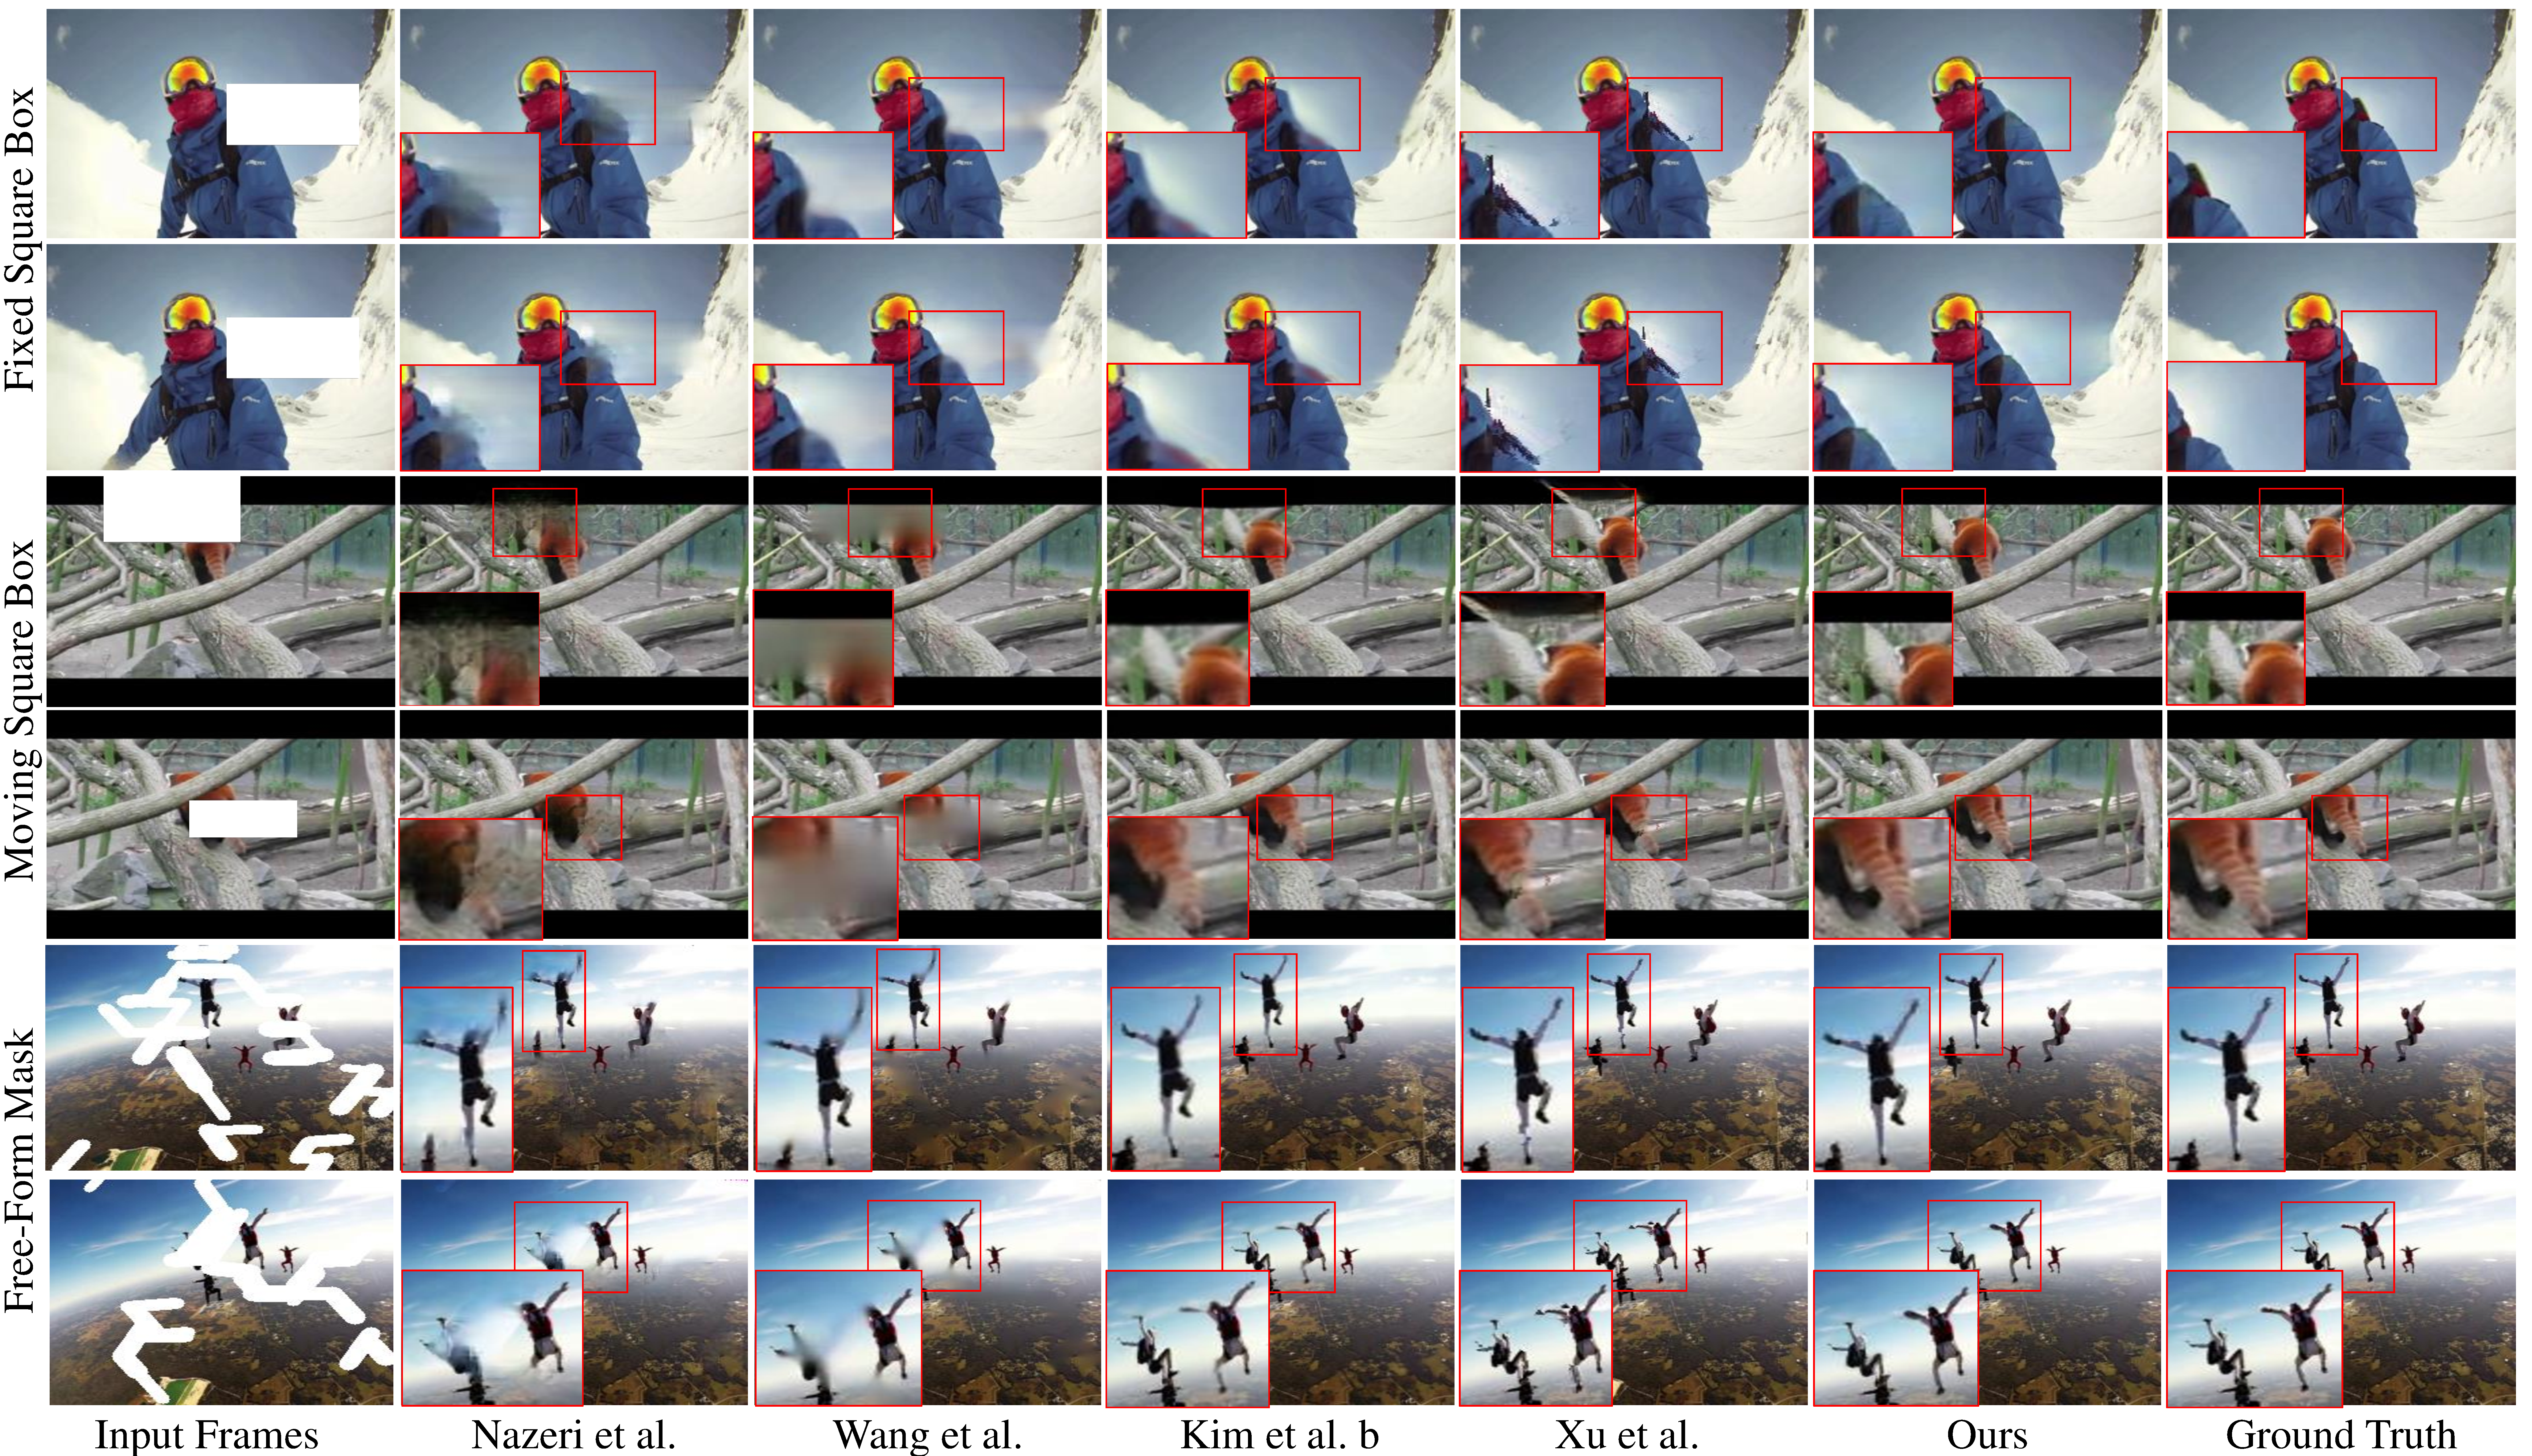
\includegraphics[scale=0.127]{viszong} % Reduce the figure size so that it is slightly narrower than the column. Don't use precise values for figure width.This setup will avoid overfull boxes. 
	\caption{Visualization for video inpainting on YouTubeVOS. Our method can produce frames with finer sturcture than existing methods. }
	\label{viszong}
\end{figure*}


\subsection{Main Results on Video Inpainting}

We compare our results with state-of-the-art inpainting methods~\cite{nazeri2019edgeconnect,wang2019video,Kim_2019_CVPR1,Xu_2019_CVPR} for the first three mask settings on the YouTubeVOS dataset. 
%
The quantitative results and running times are reported in Table~\ref{tab:sem}.
It shows that our method outperforms state-of-the-art methods on the three metrics, demonstrating the effectiveness of introducing structural guidance into video inpainting.
Moreover, our method is also very efficient on time performance. 
Our method is twice faster than \cite{Kim_2019_CVPR1} and 4 times faster than \cite{Xu_2019_CVPR}. 
%
We also show some inpainting examples in Fig.~\ref{viszong}.
Compared with existing methods, the inpainting results predicted by our method are more realistic with finer details. 
We can observe that the frames predicted by our method contains more sharper object contours. This is achieved by the effectiveness of structure information in video inpainting.
%
When looking at two neighboring frames in each video, it can be seen that our method produces more temporally smooth results. More comparisons of the completed videos can be found in the supplementary material.




Comparing with the 2D image inpainting method~\cite{nazeri2019edgeconnect} which also predicts edges first to represent 
the structural information, our method greatly increases the completion performance by leveraging neighboring frames to complete edges and synthesize textures. 
%
It demonstrates that our method is not a naive extension to utilize structure information in video inpainting.
This indicates that structure clues can bring strong promotion to video inpainting.

%% Time performance analysis 

 

\dlt{
Specifically, the additional time cost brought by edge enhancement is negligible.
%
When the flow inpainting module is removed in SOVI, the inference speed is almost twice faster, and our performance is still competitive.
}
%


\subsection{Results on Object Removal}


In regard to the fourth setting that aims to complete regions in arbitrary shapes, there is no ground truth for quantitatively evaluation. Therefore,
we conduct a user study on the DAVIS dataset to evaluate the visual quality of our method, comparing with four state-of-the-art methods \cite{nazeri2019edgeconnect,wang2019video,Kim_2019_CVPR1,Xu_2019_CVPR}.
%
In each test, we show three videos to the subject at the same time. The original video with red masks indicating objects to remove is shown in the video, while the completed result of our method and the result of another method are shown on the two sides in a random order.
%  
The subjects are allowed to watch the videos multiple times to better evaluate the differences.
For each video triplet, the subject is asked to choose which completed video is prefered.
%
In total 30 subjects participated our user study. 
Each participant watched 20 triplets carefully, and choose which inpainted video is visually better. 
%
Each method is compared for about 150 times.
%
The preference in the user study is shown in Fig.~\ref{fig:user-study}. \cxj{change table to figure.}
%
Comparing to \cite{nazeri2019edgeconnect,wang2019video,Kim_2019_CVPR1}, our results are preferred by a significant larger portion of subjects.
%
When comparing with the flow-guided method~\cite{Xu_2019_CVPR}, our method is preferred in $59.41\%$ of the tests. 
Notably, our method is much faster than ~\cite{Xu_2019_CVPR}.

\dlt{
We list the preferred proportion of each methods compared to ours. The results are reported in Table~\ref{tab:userstudy}, which shows that our method is preferred by the users. }


%
Fig.~\ref{vis_forg} demonstrates that two examples of object removal using different methods. 
%We can see that generated by our methods are visually better than existing methods.
Compared to the blurry contents in the results of \cite{nazeri2019edgeconnect,wang2019video,Kim_2019_CVPR1}, our method produces sharp object boundaries and fine visual details. 
Though the completed contents using \cite{Xu_2019_CVPR} have shape edges, the global structure is corrupted on the human bodies. In comparison, our method achieves more complete and plausible structure with fine details.



\begin{table}[t]
	\caption{The result of user study. \cxj{Change table to figure.}}\smallskip
	\tiny
	\centering
	\resizebox{0.7\columnwidth}{!}{
		\smallskip\begin{tabular}{c|c}
			\hline
			Comparing Methods&Preferred Proportion\\
			\hline
			Ours/Nazeri et al.&0.9083/0.0917\\
			\hline
			Ours/Wang et al. &0.8015/0.1985\\
			\hline
			Ours/Kim et al. b &0.7357/0.2643\\
			\hline
			Ours/Xu et al. &0.5941/0.4059\\
			\hline
			
			
		\end{tabular}
	}
	\label{tab:userstudy}
\end{table}




\subsection{Ablation Study}
To demonstrate the effectiveness of each proposed component in our approach, we conduct a series of ablation studies on the YouTubeVOS dataset with the first three mask settings. 
%
We test four variants of our model. 
The baseline model STINet only consists of the coarse-to-fine texture inpainting network without using the edge maps as input and no SAM in the refinement module.
This model simply integrates neighboring frames to predict the missing content for the current frame.
%
Then we add the edge inpainting network and fed the texture inpainting network with the completed edge maps to get the second model `+ENet'.
The third model `+SAM' is constructed by adding the structure attention module on the second model. 
Finally, we add the flow guidance including FNet and the ensemble module to get our full model `+Flow'.
The quantitative results are reported in Table~\ref{tab:sem}. 


\subsubsection{Effect of Structure Clues in TexNet.}


\begin{figure}[!ht]
	\centering
	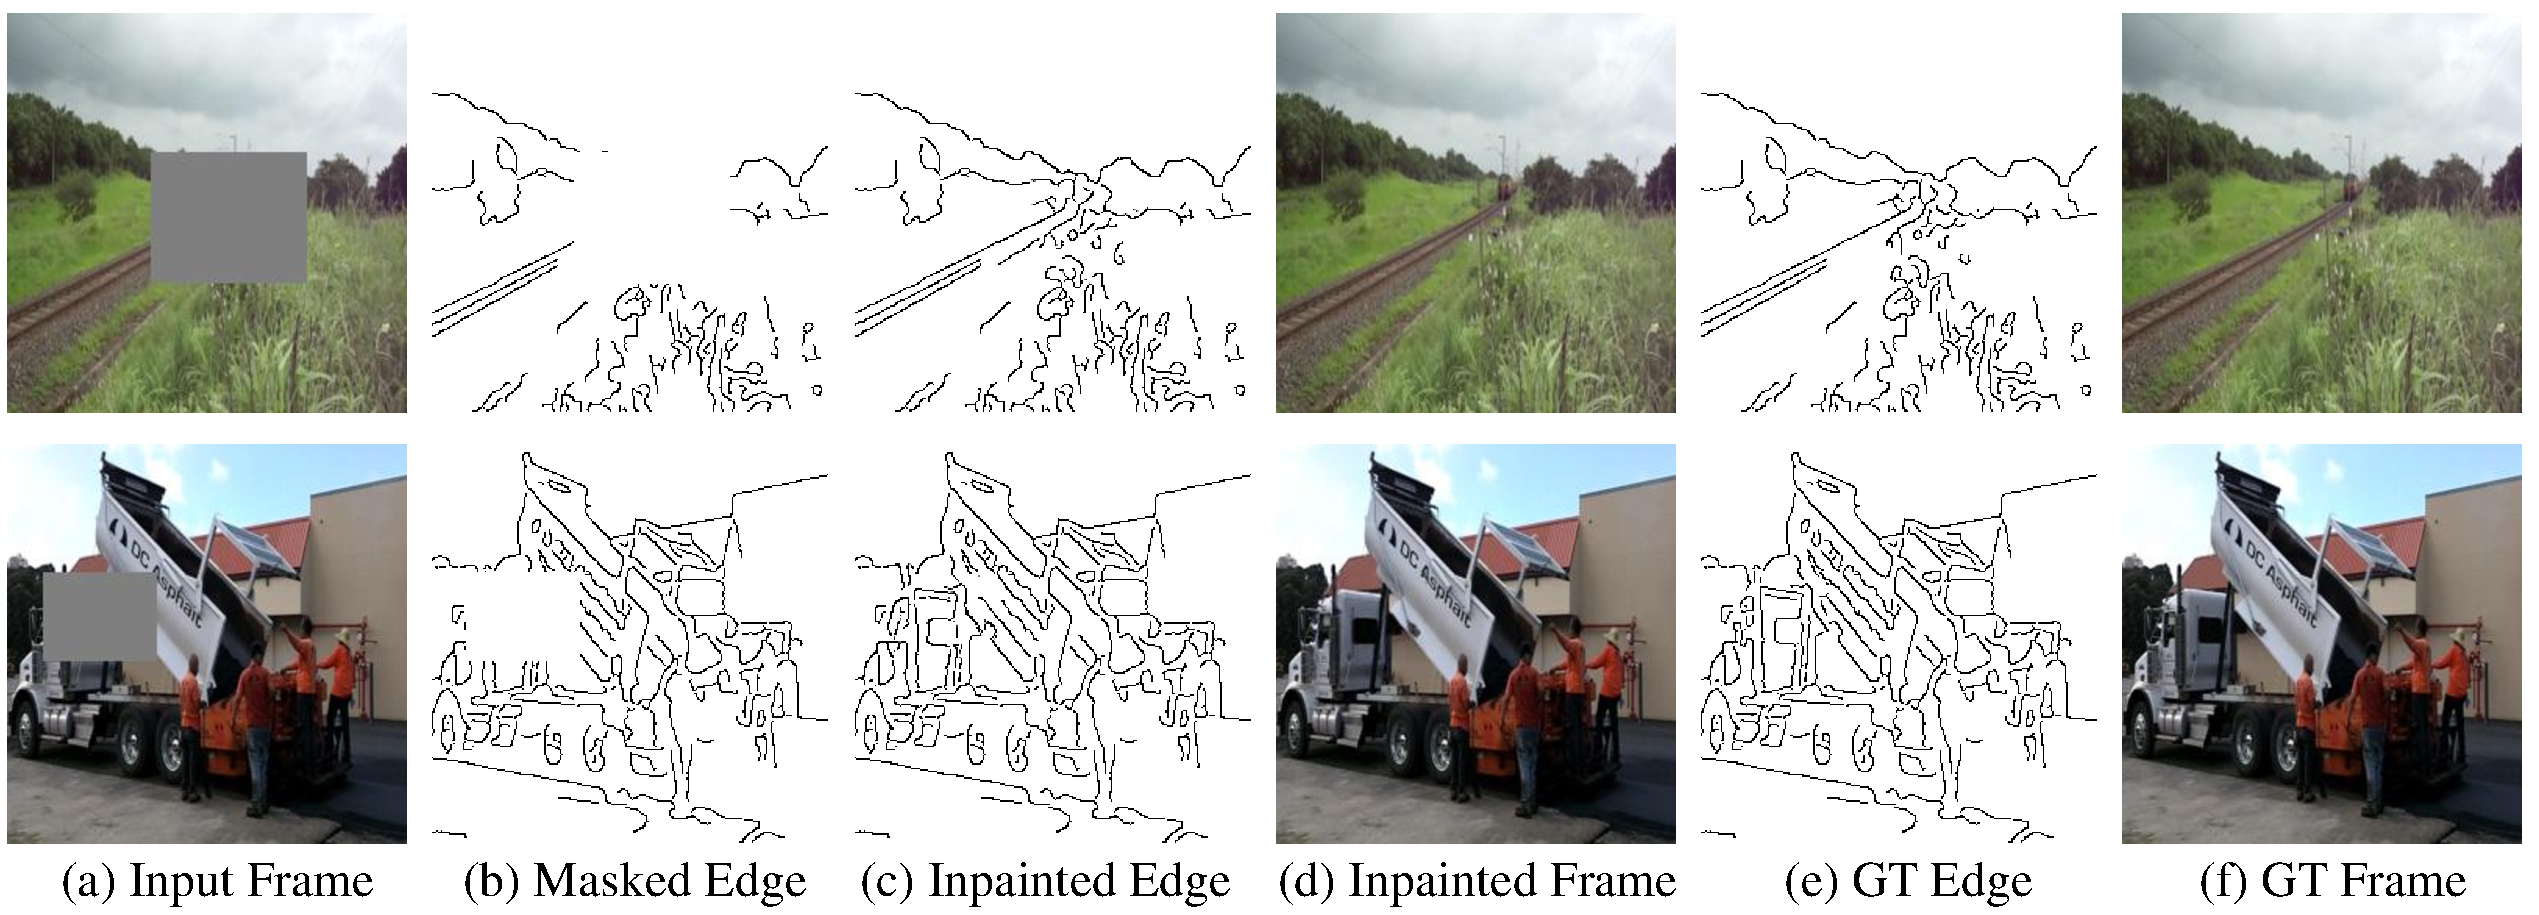
\includegraphics[width=0.97\columnwidth]{edgevis} % Reduce the figure size so that it is slightly narrower than the column. Don't use precise values for figure width.This setup will avoid overfull boxes. 
	\caption{Visualized effects of exploring structure edges in video inpainting. It's obvious that we can obtain more detail-clear results with structure guidance.}
	\label{edgevis}
\end{figure}


\dlt{
To evaluate the effects of structural information in video inpainting, we successively add different parts to the baseline and compare their performances. 
Three variants are used: 'Baseline', '+ENet', and '+SAM'. 
'STI' is the baseline using only texture inpainting network, without either structure clues or temporal information. '+edge input' is the model that uses the predicted edge maps as input. `+SAM' is the model to which structure attention module is applied.
}

%As shown, the network achieves better results when edge information is utilized, comparing '+edge input' to 'STI'. It indicates that edge clues are effective guidance in video inpainting, which helps the network to predict more accurate frames.
Comparing the four variants, `+ENet' brings large improvement over the baseline model.
It indicates that sparse edges provide effective structural guidance in video inpainting.
% which helps the network to predict accurate missing content.
When we further add SAM to STI, extra improvement is obtained. 
It demonstrates that the spatial correlation between  edges and textures can be better embedded and absorbed by the texture inpainting network than simply feeding the completed edge maps as extra channels into TexNet.
%The above analyses prove that the edge clues are effective guidance in video inpainting, which helps the network to predict more accurate frames.


Fig.~\ref{edgevis} shows the results generated using the three variants. 
It's obvious that after introducing the edge structure, the inpainted frames become visually better with sharper object contours. 
Besides, the edge maps predicted by our method are reasonable and clear, which well represents the structure information and show the strong edge inpainting ability of ENet. Thus, it is crucial to explore structural details when inpainting the videos.




%\begin{figure}[t]
%	\centering
%	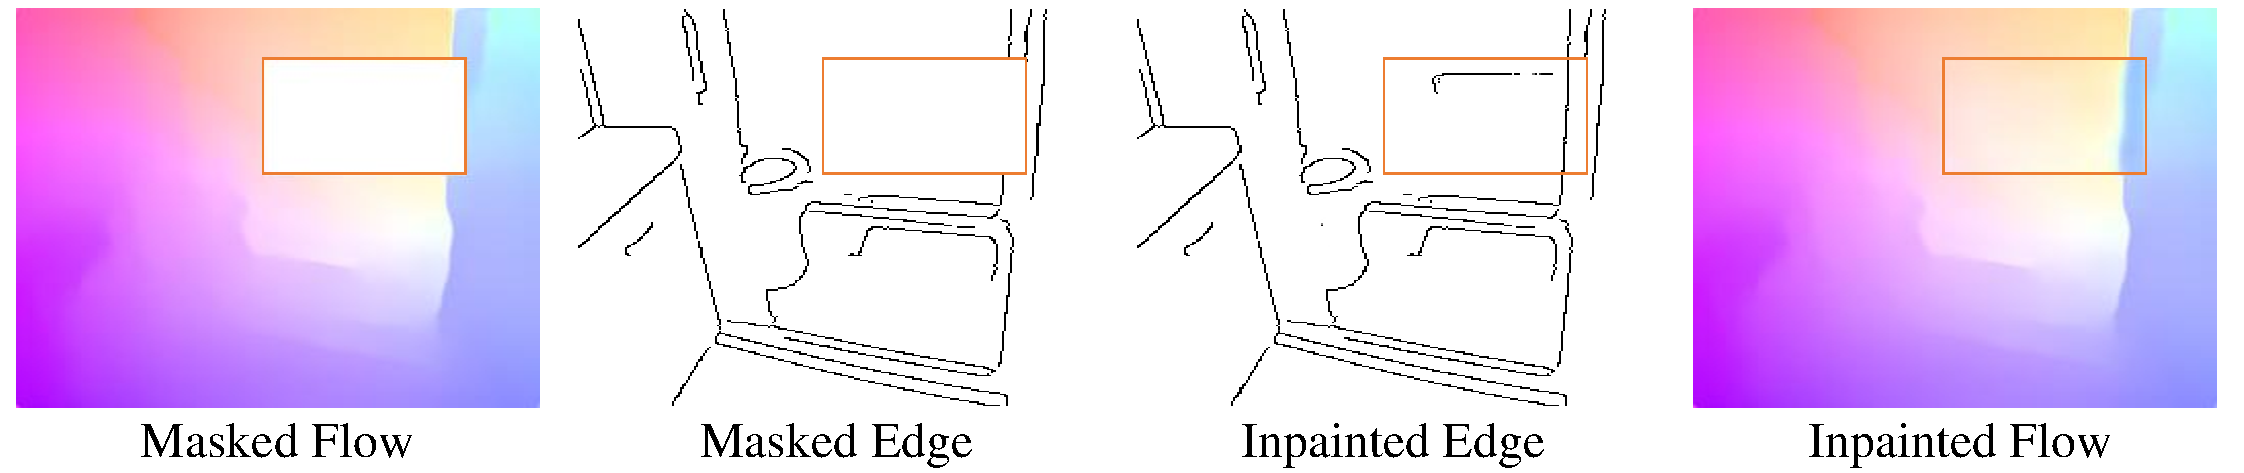
\includegraphics[width=1.0\columnwidth]{flowvis} % Reduce the figure size so that it is slightly narrower than the column. Don't use precise values for figure width.This setup will avoid overfull boxes. 
%	\caption{Visualized optical flow predicted by our method.}
%	\label{flowvis}
%\end{figure}
\begin{figure}[t]
	\centering
	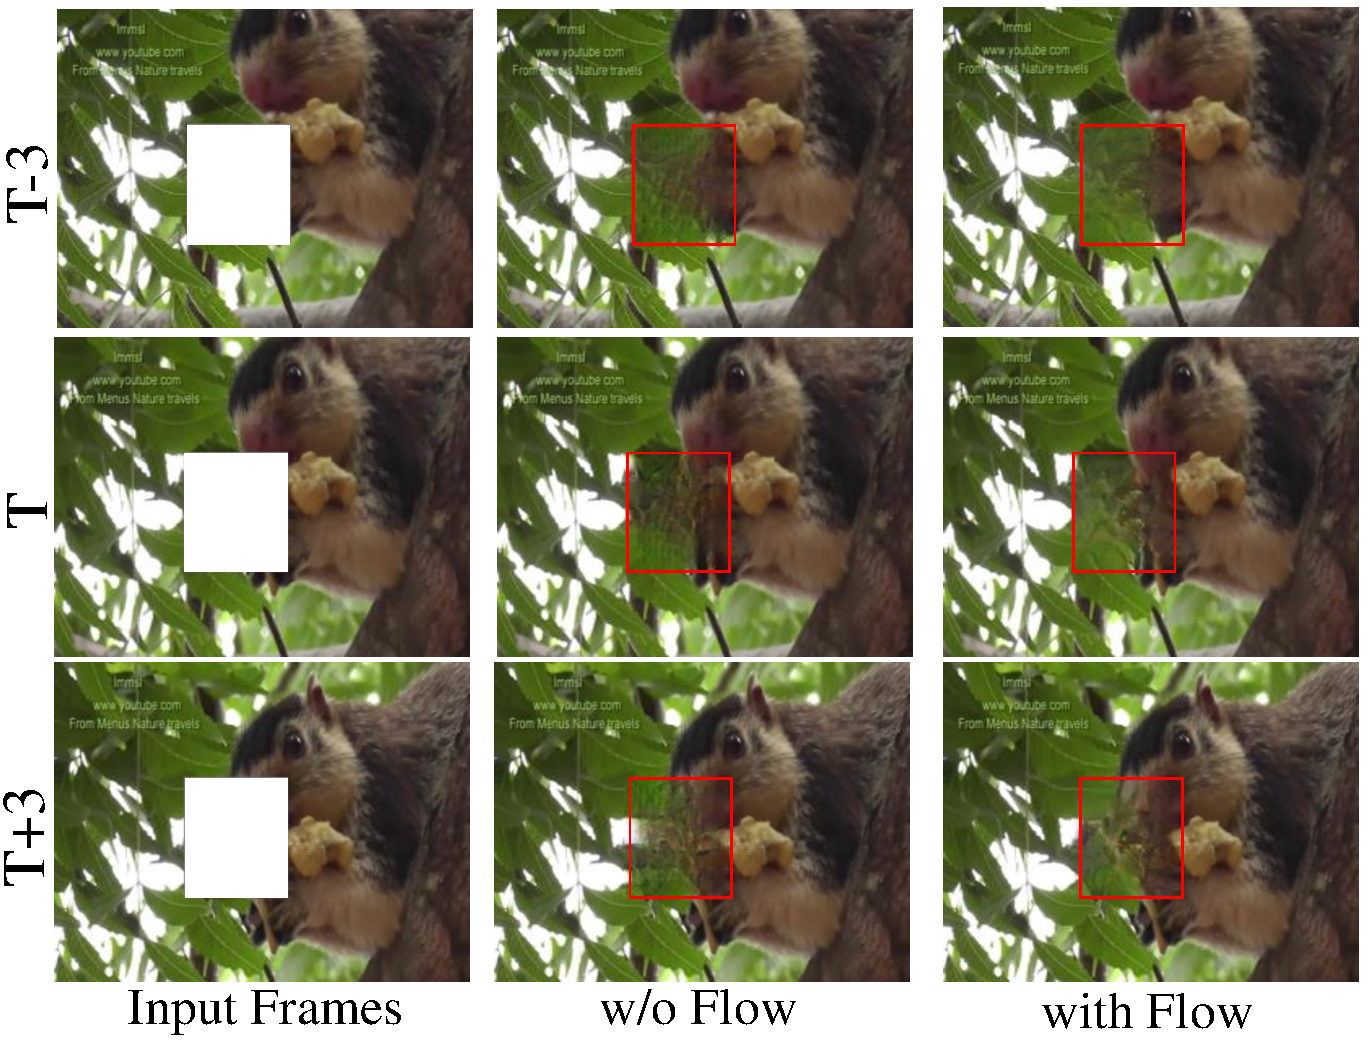
\includegraphics[width=1.0\columnwidth]{flow_vis} % Reduce the figure size so that it is slightly narrower than the column. Don't use precise values for figure width.This setup will avoid overfull boxes. 
	\caption{Visualized effects of temporal information.}
	\label{flow_vis}
\end{figure}

\subsubsection{Effect of Temporal Information in TexNet.}

Temporal consistency is also an important factor in video inpainting. 
In our method, we utilize temporal information from the inpainted flows to smoothen artificial flickers via the developed flow-guided warping and temporal ensemble module. 
From Table~\ref{tab:sem}, we can see that the quantitative performance is slightly improved on all the three settings by adding the flow guidance. 
As shown in Fig.~\ref{flow_vis}, the synthesized contents in neighboring frames are more consistent in time.
%and the color changes between neighboring frames become less obvious after employing flow.
Furthermore, it should be noted that the performance improvement from temporal information is smaller than that from structure information in this paper.
The reason maybe that our base model has certain ability to utilize complementary information of neighboring frames.
%Both the quantitative and qualitative results prove that the motion information is beneficial to temporal consistency as well as inpaitning.


\dlt{
%We use '+flow' to denotes the model 
First of all, we provide the visualized results in Fig.~\ref{flowvis}, where the proposed FNet can effectively complete the missing flows with fine boundaries.


%`Ours' denotes our full model that utilizes flow-guided warping for training and the temporal ensemble module.
It can be seen that the result is further improved after utilizing temporal information. It proves that the complementary contents can be aggregated by motion, which is helpful in video inpainting. 
}


%a flow warping loss to smoothen the artificial flickers and propagate complementary information from neighboring frames. 
%It is achieved by $\mathcal{L}_{fec}$, which demonstrates that structure information can also boost the completion of optical flow.
%To evaluate the impact of temporal smoothening in STI, we compare two baselines, STI and STI w/o flow.
%As shown in Table~\ref{tab:edge}, STI works better than STI w/o flow, values...!!!.
%The visualized results are shown in Fig.~\ref{flow_vis}.
%It can be observed that the artificial flickers are alleviated when motion guidance is involved. 

%Besides, he visulization results in Fig.~\ref{flowvis} shows that $\mathcal{L}_{fec}$ encourages the network to predict optical flow  which demonstrates that structure information can also boost the completion of optical flow.

%We only use the first three mask settings on YouTubeVOS.
%\cxj{for what reason? page limit of the paper? How about others? Can we result in the same conclusion for different mask settings?}


%We discussed four variants of our method. We 
%\begin{enumerate}
%	\item STI: The Spatio-Temporal Inpainting network without guidance of either edge or flow.
%	\item +edge:
%	\item Free-from mask. We apply irregular mask which imitates hand-drawn masks on each frame, following \cite{liu2018partialinpainting}. 
%	\item Foreground object mask. This type of masks are defined to line out the foreground objects in videos, which is used for object removal.
%\end{enumerate}
%\noindent \textbf{Baselines.} Several variants of STSENet are defined as following. (1) STI w/o flow: The Spatio-Temporal Inpainting network without flow guidance \cxj{with or without EdgeNet and SEM?}. (2) STI w/o edge: The Spatio-Temporal Inpainting network without structure guidance. (3) STSENet w/o $\mathcal{L}_{fec}$: The Spatio-Temporal Inpainting network with guidance of both structure and motion, but $\mathcal{L}_{fec}$ is not used. (4) STSENet is the model which uses all modules proposed in this paper. 
%
%\cxj{We discussed four variants of our method. Use that version. }
\begin{figure}[!h]
	\centering
	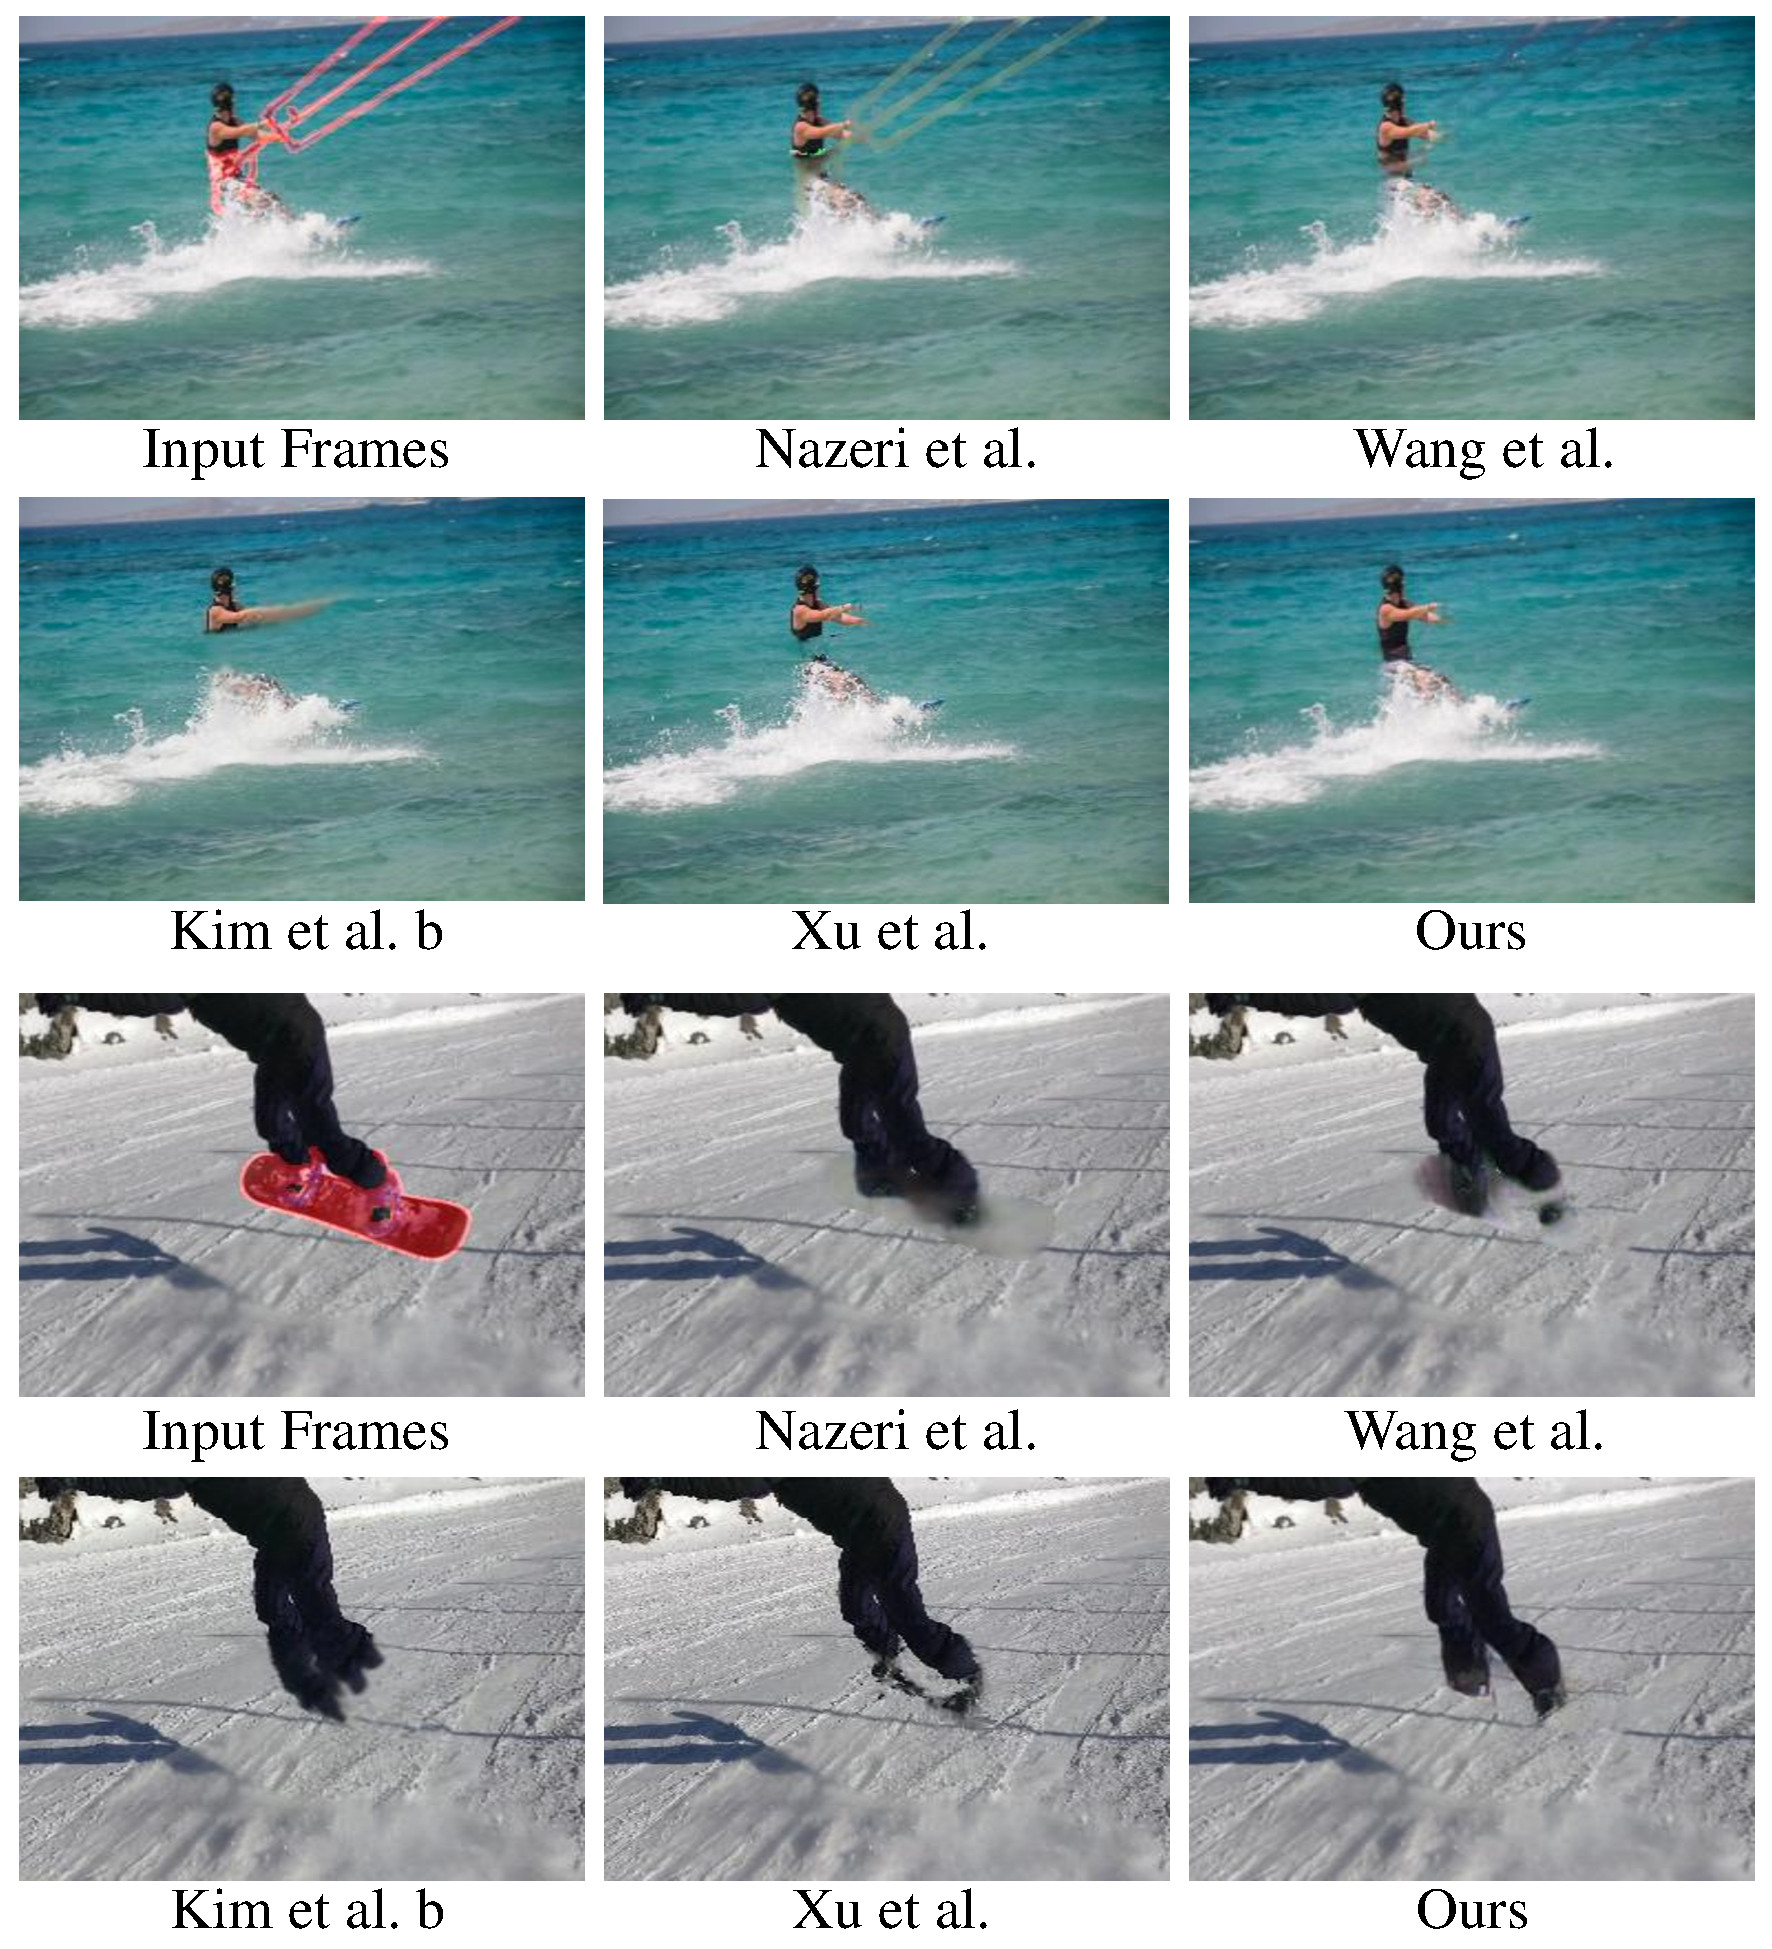
\includegraphics[width=1.0\columnwidth]{vis_forg} % Reduce the figure size so that it is slightly narrower than the column. Don't use precise values for figure width.This setup will avoid overfull boxes. 
	\caption{Visualized object foreground removal. The red mask in input frames indicates the object that we want to remove.}
	\label{vis_forg}
\end{figure}














 

